\chapter{Domain Driven Design}

\section{Analyse der Ubiquitous Language}

\paragraph{Sprache} Als Sprache der Ubiquitous Language standen Deutsch und Englisch zur Auswahl. Da die Domänenexperten die Domäne ebenso gut in englischer wie in deutscher Sprache beschreiben können, Englisch jedoch von wesentlich mehr Personen und Entwicklern verstanden wird als Deutsch, wurde Englisch als Sprache für die Ubiquitous Language gewählt.

\paragraph{Wesentliche Begriffe} Da die Domäne der Applikation im Wesentlichen die Themen Kochrezepte und Lebensmittel betrifft und es sich hierbei um Gebiet handelt, welches auch in der englischen Sprache präsent ist, können für die zentralen Begriffe der Domäne die im Englischen üblichen Begriffe verwendet werden. 

Ein zentrales Konzept der Domäne ist das Kochrezept. Ein Kochrezept wird in der Ubiquitous Language mit dem Begriff \enquote{Recipe} bezeichnet. Ein Recipe besitzt typischerweise eine Liste von Zutaten, welche in der Domäne als \enquote{Ingredient} bezeichnet werden. Eine Ingredient bezeichnet ein Nahrungsmittel, von dem für ein Rezept eine bestimmte Menge verwendet wird, welche in einer bestimmten Einheit gemessen wird. Dieses Nahrungsmittel wird als \enquote{Food} bezeichnet, die verwendete Menge als \enquote{Quantity} und die entsprechende Einheit als \enquote{Unit}.

Das zweite zentrale Konzept der Domäne ist das Benutzerprofil, welches in der Ubiquitous Language als \enquote{Profile} bezeichnet wird. Zu einem Profile gehört, wie in der Einleitung erwähnt, eine Menge vorrätiger Foods. Neben den vorrätigen Foods gehören zu einem Profile auch die Meinungen des Nutzers zu bestimmten Lebensmitteln, welche als \enquote{Opinions} bezeichnet werden. Diese Opinion des Nutzers kann sieben Stufen annehmen: \enquote{Foodgasm}, \enquote{Love}, \enquote{Like}, \enquote{Indifferent}, \enquote{Dislike}, \enquote{Hate} und \enquote{Dealbeaker}, hier in zunehmender Reihenfolge der Abneigung des Nutzers gegenüber dem betreffenden Lebensmittel.

\section{Entities \& Value Objects}

\begin{figure}[ht!]
    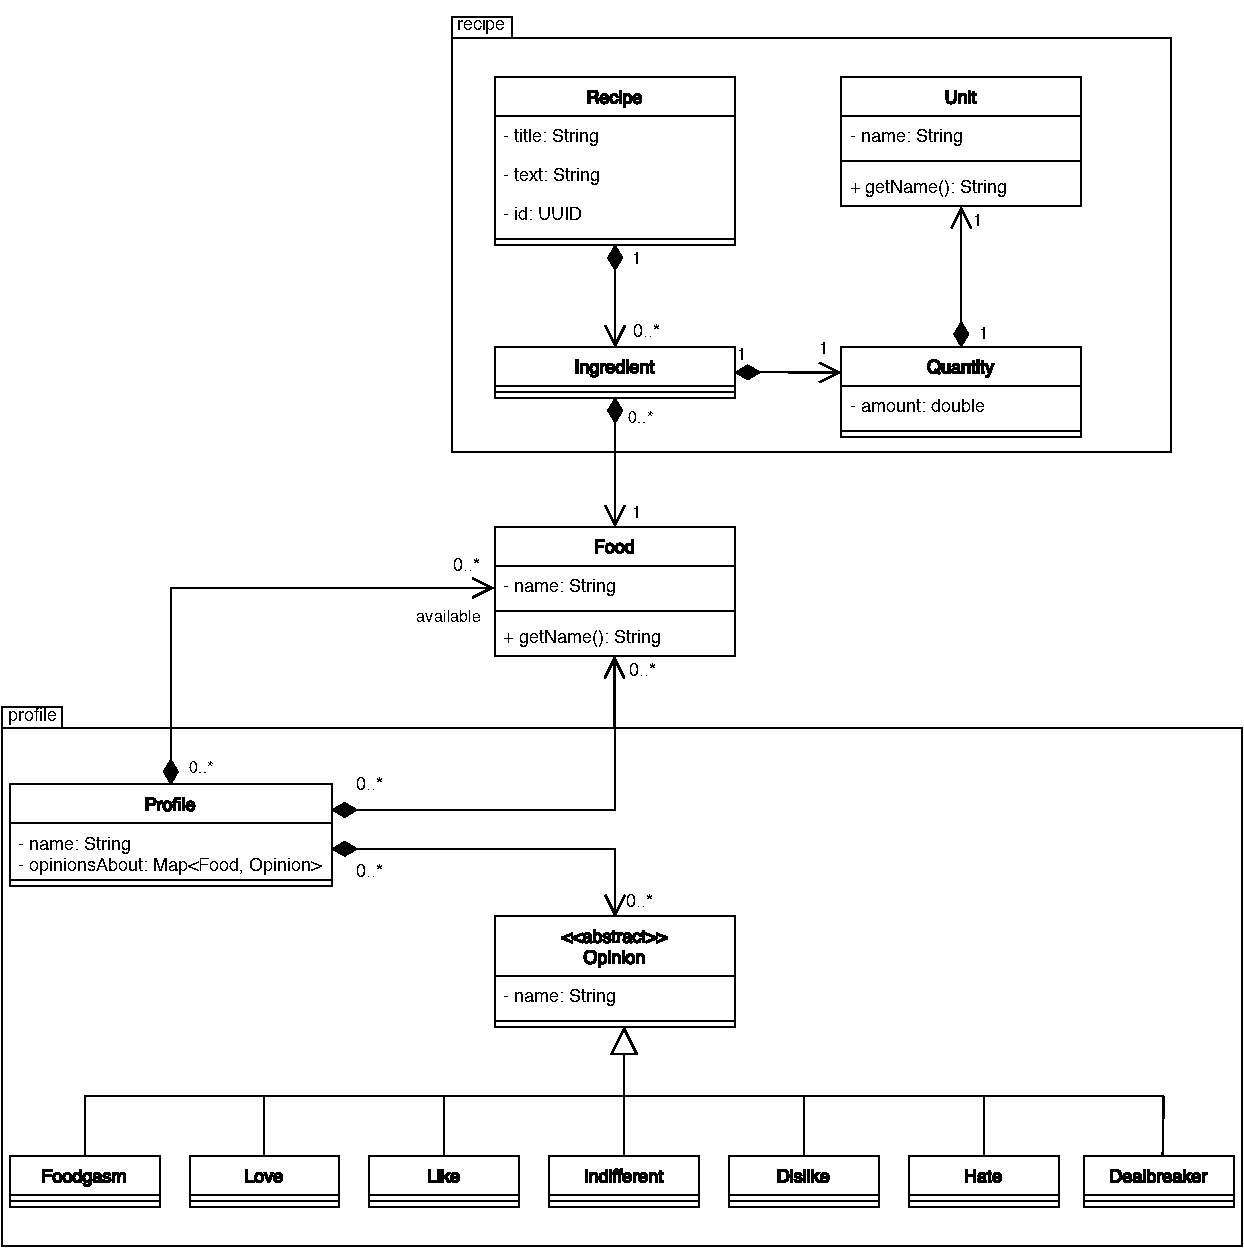
\includegraphics[width=0.98\columnwidth]{../diagrams/entity_uml.pdf}
    \caption{Klassendiagramm der Domäne}
    \label{fig:class-diag-domain}
\end{figure}

\autoref{fig:class-diag-domain} zeigt das Klassendiagramm der Domäne. Im Package recipe existiert eine Entity: das Recipe. Jedes Recipe besitzt durch eine UUID eine eigene Identität. Außerdem können Rezepte in seltenen Fällen auch nachträglich abgewandelt werden und besitzen daher grundsätzlich veränderliche Werte. Bei der Ingredient hingegen handelt es sich um ein Value Object, da diese keine eigene Identität besitzt. Existieren zwei Ingredients mit dem gleichen Food und der gleichen Quantity, so sind diese gleich. Außerdem ist ihr Zustand unveränderlich, so wird etwa bei einer Änderung in einem Rezept die betreffende Ingredient gelöscht und eine neue erstellt. Ebenso verhält es sich mit der Quantity: Sind Amount und Unit einer Quantity gleich, so sind auch die Quantities gleich und auch ihr Zustand ist unveränderlich. Zuletzt enthält das Package noch die Unit. Auch hier handelt es sich um ein Value Object, da auch die Gleichheit von Units lediglich von ihren Werten, also von ihren Namen abhängt. Ebenso besitzt eine Unit keinen eigenen Lebenszyklus und ihr Zustand ist unveränderlich.

Auch im Package profile existiert eine Entity: das Profile. Jedes Profile besitzt durch seinen Namen eine eigene Identität, da auch zwei Profiles mit gleichem vorhandenen Food und gleichen Opinions zu verschiedenen Nutzern gehören können und daher unterscheidbar sein müssen. Die auch die Unterklassen der abstrakten Klasse Opinion, welche die möglichen Opinions eines Nutzers über ein Food abbilden, repräsentieren Value Objects, da sie weder eine eigene Identität noch veränderliche Werte besitzen. Da sie außerdem keine Attribute besitzen, wird ihre Gleichheit nur über ihren Typ bestimmt. Die Verbindung zwischen Food, Profile und Opinion wird durch OpinionAbout hergestellt. Es handelt sich auch hier um eine Value Object, da auch eine OpinionAbout weder einen eigenen Lebenszyklus noch eine Identität besitzt, da sie durch ihre Werte, also das Food und die zugehörige Opinion, definiert wird. Solle ein Nutzer seine Meinung zu einem Food ändern, so wird die bestehende gelöscht und eine neue erzeugt.

Zwischen den beiden Packages steht das Food, da es sowohl vom Profile als auch von der Ingredient verwendet wird und daher keinem der Packages eindeutig zugeordnet werden kann. Auch bei Food handelt es sich um ein Value Object, da es ebenfalls nur durch eine Werte definiert wird: Zwei Foods mit gleichem Namen sind gleich, daher besitzt es keine eigene Identität und da sich der Name auch nicht ändern wird, besitzt es auch keinen erkennbaren Lebenszyklus. 

\section{Aggregates}
Da alle Klassen im Package recipe Eigenschaften eines Recipe abbilden, werden diese, also die Klassen Recipe, Ingredient, Unit, Quantity und Unit, zu einem Aggregate zusammengefasst. Die Root Entity ist dabei das Recipe selbst.

Ähnlich verhält es sich im Package profile: Auch hier bilden alle Klassen direkt oder indirekt Eigenschaften des Profiles ab, daher werden auch diese, also die Recipe, Food, OpinionAbout und Opinion bzw. deren Unterklassen zu einem Aggregate zusammengefasst. Die Root Entity ist hier das Profile.

Die Klasse Food nimmt eine Sonderstellung ein: Da sie von beiden Aggregates verwendet wird und daher zuvor auch schon keinem Package eindeutig zugeordnet werden konnte, ist sie Teil beider Aggregates.

\section{Repositories}
Für den Zugriff auf den persistenten Speicher werden zwei Repositories gemäß dem Grundsatz \enquote{Ein Repository pro Aggregate} definiert: Das ProfileRepository erlaubt den Zugriff auf das Profile, also die Root Entity des entsprechenden Aggregates. Analog hierzu ermöglicht das RecipeRepository Zugriff auf das Recipe als Root Entity des zugehörigen Aggregates. 
